\documentclass[12pt,a4paper]{article}

% Quelques options d'encodage, de langues et de format du document
\usepackage[utf8]{inputenc}
\usepackage[T1]{fontenc}
\usepackage[english]{babel}
\usepackage[top=2cm, bottom=3cm, left=1.75cm, right=1.75cm]{geometry}
\usepackage{setspace}

\usepackage{graphicx} % Pour la commande "\includegraphics"
\usepackage[ % Modified parameters
    bookmarks,
    colorlinks,
    citecolor=black,
    urlcolor=blue,
    linkcolor=black,
    pdfpagemode=UseNone
]{hyperref} % Pour la commande "\url"

\pagenumbering{arabic}

% ------------------------------------------------------------------
% CITATION MANAGEMENT
% ------------------------------------------------------------------

% APA Style
\usepackage{cite}
\bibliographystyle{apalike}

\renewcommand\refname{Bibliography}

% Proper formatting and line breaking for URLs
\usepackage{url}

% Change "References" to "Bibliography"
\usepackage{etoolbox}
\patchcmd{\thebibliography}{\section*{\refname}}{\section*{Bibliography}}{}{}

% ------------------------------------------------------------------
% SUBFIGURE MANAGEMENT
% ------------------------------------------------------------------

\usepackage{subcaption}
\usepackage{pgfplots}
\usepackage{booktabs}

% ------------------------------------------------------------------
% COLORED TEXT MANAGEMENT
% ------------------------------------------------------------------

\usepackage{xcolor}
\usepackage{todonotes}
\setuptodonotes{inline=always}

% ------------------------------------------------------------------
% CODE MANAGEMENT
% ------------------------------------------------------------------

\usepackage{listings}

\lstdefinelanguage{Cypher}{
    morekeywords={
        MATCH, RETURN, WHERE, CREATE, DELETE, SET, MERGE, DETACH,
        WITH, LIMIT, SKIP, ORDER, BY, DESC, ASC, OPTIONAL, CALL
    },
    sensitive=true,
    morecomment=[l]{//},
    morecomment=[s]{/*}{*/},
    morestring=[b]',
    morestring=[b]"
}

% Listing style for better readability
\lstset{
    language=Cypher,
    basicstyle=\ttfamily\small,
    keywordstyle=\color{blue},
    stringstyle=\color{orange},
    commentstyle=\color{gray},
    showstringspaces=false,
    numbers=left,
    numberstyle=\tiny,
    breaklines=true,
    frame=single
}

\begin{document}

\begin{center}
    \begin{tabular}{|p{0.2\textwidth}|p{0.75\textwidth}|}
        \hline
        {
            \vspace{0cm} % without it, bugs, don't know why?
            \centerline{
\includegraphics[width=\linewidth]{./images/tp-ipp.png}}
        }
         & {
                \vspace{0cm} % same here
                \centering
                \large
                {\hfill January, 2025}

                \vspace*{.5cm}
                \textbf{APM\_5AI29\_TP}

                \vspace*{.5cm}
                \setstretch{1.5}
                {\Large\textbf{Language Models and Structured Data}}

                \vspace*{.5cm}
                Mid-term Project Report

                \vspace*{1cm}
        }    \\
        \hline
    \end{tabular}
\end{center}

\noindent Acronym of the Team: AWESome\\
Names: Mochamad \textbf{Ardi}ansyah Nurgaha; \textbf{Will}iam Liaw; \textbf{Eddie} Groh; \textbf{Sri} Raam Appakutti Palani

    {\centering\rule{\linewidth}{.5pt}}

\begin{center}
    \section*{Multi-class link prediction with PyKEEN and Large Language Models}
\end{center}

\section*{Abstract}

% 2/3 lines

This report explores the performance of knowledge graph embedding models for link prediction, focusing on a comparative analysis between PyKEEN's embedding models and large language model (LLM)-based approaches.
Using the Hetionet biomedical knowledge graph as a testbed, we evaluate the predictive capabilities of various PyKEEN models and introduce a novel method that leverages Llama embeddings, with and without retrieval-augmented generation (RAG), to enhance link prediction.

\section*{Problem Statement}

% Explain which problem (and task) you're addressing. It should be framed as a problem (typically something desirable we want, or something undesirable we don't want, or something we don't understand, or something surprising).

Knowledge graphs are valuable tools for representing complex relationships between entities. However, a significant challenge arises from their inherent incompleteness, as many potential connections between entities are missing. This lack of information limits the utility and accuracy of downstream applications such as recommendation systems, biomedical research, and drug repurposing, which is an initial departing point for the present academic work.

The objective of this project is to address this issue by employing knowledge graph embedding techniques through PyKEEN~\cite{pykeen} to predict and classify missing links, thereby enriching the graph. Additionally, the project explores how large language models (LLMs) could further enhance or complement traditional embedding-based approaches. We intend to investigate several LLM-based methods, including zero-shot, few-shot, and retrieval-augmented generation (RAG), to assess their effectiveness in knowledge graph completion tasks.

% \todo{LLM integration remains a future step. (SOMEONE STILL NEEDS TO IMPLEMENT IT AND CHANGE THIS SECTION}


In this project, we focus on link prediction task for knowledge graphs 
(KGs). Given incomplete triple in a KG \((h, r, ?)\) or \((?, r, t)\), 
the goal is to predict the missing entity, either it is head \(h\) 
or tail \(t\), where \(h, t \in E\) and \(r \in R\), E denotes set of 
entities, R denotes set of relations. The model that we used follows 
KICGPT \cite{wei2023kicgpt} with modification on the LLM used. 

\subsection{Architecture}
\label{sec:method:architecture}

\begin{figure}
    \centering
    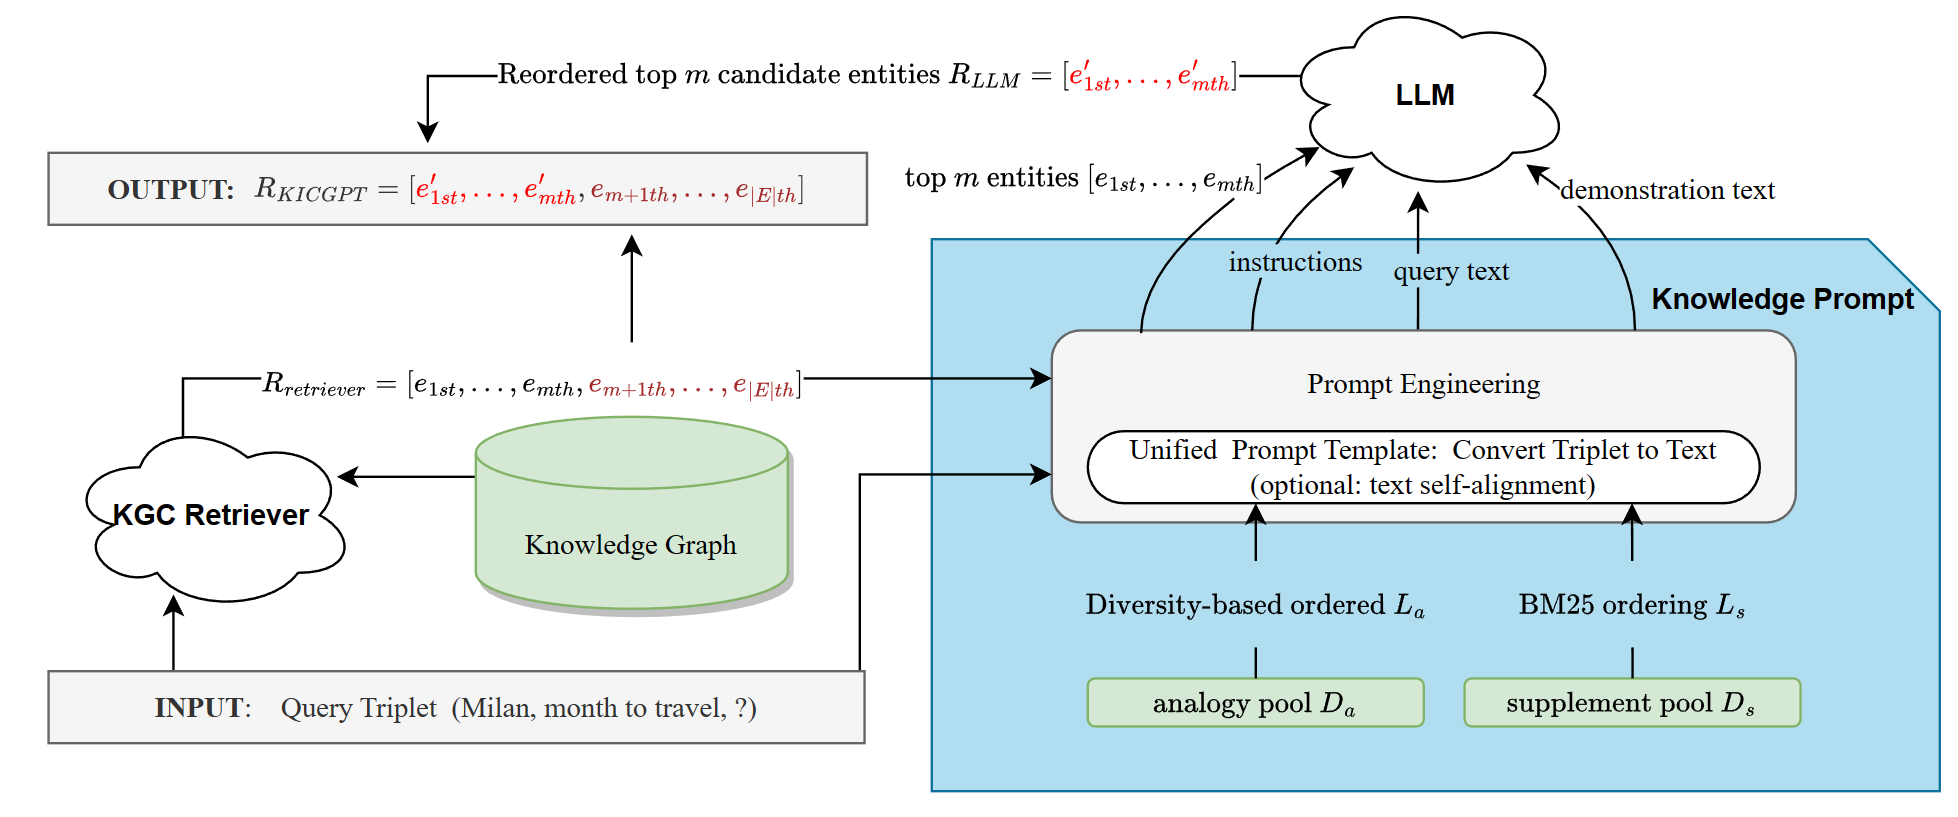
\includegraphics[width=0.8\textwidth]{figures/arc3.png}
    \caption{KICGPT Architecture \cite{wei2023kicgpt}}
    \label{fig:KICGPTarchitecture}
\end{figure}

KICGPT primarily covers three main components as can be seen in Figure 
\ref{fig:KICGPTarchitecture}, which are a triple-based KGC retriever, 
the Knowledge Prompt, and a LLM. For each query triple \((h, r, ?)\), 
the KGC retriever retrieves the score of \((h, r, e)\) for each entity 
\(e \in E\) in descending order 
\(R_{retriever} = [e_1, e_2, ..., e_{|E|}]\). 
Using prompt engineering in the Knowledge Prompt, LLM performs reranking 
of the top \(m\) entities 
\(R_{LLM} = [e^{'}_1, e^{'}_2, ..., e^{'}_m]\). Finally, KICGPT will 
output final ranking of top m entities from the LLM and the rest of
the entities from the KGC retriever 
\(R_{KICGPT} = [e^{'}_1, e^{'}_2, ..., e^{'}_m, e_{m+1}, ..., e_{|E|}]\)

\subsubsection{Knowledge Prompt}
Knowledge Prompt is introduced in KICGPT as in-context learning
strategy to provide context to the LLM by integrating part of the KG
into the demonstration. There are two pools of triples in the 
demonstration, analogy pool \(D_a\) and supplement pool \(D_s\). 
To help the LLM understand the query triple, the analogy pool contains 
triples with the same relation \(r\) as the query \((h, r, ?)\), 
\(D_a = \{(e^{'}, r, e^{"}) \in G_{train} \cup G_{valid} \mid e, e^{"} \in E\}\).
In addition, the supplement pool contains triples with one of its entity 
(tail or head) is the same as the query's head \((h, r, ?)\),
\(D_s = \{(h, r, e^{'}) \in G_{train} \cup G_{valid} \mid r^{'} \in R, e^{'} \in E\} \cup
\{(e^{'}, r, h) \in G_{train} \cup G_{valid} \mid r^{'} \in R, e^{'} \in E\}\).
This is to provide additional information of the query's head to the LLM.

The ordering of the demonstration is important as it affects the LLM performance.
For the analogy pool, each entity starts with a zero counter. 
A random triple from \(D_a\) is chosen first, increasing its entities'
counters by 1. Next, the triple with the lowest summed counter values 
is selected, repeating until all triples are used. The final ordered 
list is denoted \(L_a\). The supplement pool \(D_s\) provides additional context 
for the query's head entity \(h\), prioritizing relevant demonstrations. 
To achieve this, triples in \(D_s\) are ranked based on their BM25 scores, 
which measure their textual similarity to the query. The final ordered list, 
denoted \(L_s\), includes all triples from \(D_s\).

\subsubsection{Prompt Engineering}

To adapt structured triples into natural language input, KICGPT uses 
a unified prompt template, ensuring consistent formatting for queries 
and demonstrations. The interaction with the LLM follows a multi-round 
process. First, the responsibility description stage clarifies the LLM's 
role in ranking candidate answers. Next, in the question and demonstration 
description stage, the query is presented along with an explanation of 
two demonstration types: analogy-based and supplementary examples.

In the demonstration input stage, batches of demonstrations from the 
analogy \(L_a\) and supplement \(L_s\) pools are provided, repeated 
as much as the token limit allows to maximize knowledge inclusion. 
Finally, during the final query and re-ranking stage, the LLM ranks 
the top-m candidate entities, producing an ordered list \(R_{LLM}\), 
which replaces the top-m results from the retriever to generate the 
final answer.

\section*{Experimentation}

% \begin{itemize}
%     \item Dataset \& Dataset Statistics
%     \item Experimental Results based on Evaluation Metrics
%     \item Error Analysis
% \end{itemize}

This section outlines the dataset used for knowledge graph completion, presents the results of the experiments conducted using PyKEEN and LLMs.
It also provides a comparison of the models' performance based on evaluation metrics such as Mean Reciprocal Rank (MRR), Hits@K, and Mean Rank (MR).

\subsection*{Dataset and Statistics}

The Hetionet dataset~\cite{hetionet} serves as the initial foundation for this project, providing a structured biomedical knowledge graph
that integrates data from various sources to represent relationships like \textit{treats}, \textit{binds}, and \textit{causes} between genes,
compounds, diseases, and other biological entities.
While Hetionet offers a diverse and well-documented schema, its role in this project is primarily exploratory.
As we compare knowledge graph completion approaches using PyKEEN and large language models (LLMs), the dataset serves as a valuable testbed for initial experiments.
However, Hetionet may present a worst-case scenario for LLM embeddings, as many compound names are rare in natural language datasets.
Additionally, the augmentation data from Wikidata is often highly repetitive and consists mostly of basic factual information.

Key dataset statistics are summarized in Table~\ref{tab:dataset_stats}.

\begin{table}[ht]
    \centering
    \caption{Dataset Statistics (Hetionet Subset)}
    \begin{tabular}{l c}
        \hline
        \textbf{Statistic}    & \textbf{Value} \\
        \hline
        Nodes (Entities)      & 22634          \\ % MATCH (n) RETURN count(n) AS Nodes
        Relationships (Edges) & 561721         \\ % MATCH ()-[r]->() RETURN count(r) AS Relationships
        Unique Relation Types & 10             \\ % MATCH ()-[r]->() RETURN count(DISTINCT type(r)) AS UniqueRelationTypes
        Unique Triples        & 561721         \\ % MATCH (h)-[r]->(t) RETURN count(DISTINCT [id(h), type(r), id(t)]) AS UniqueTriples
        \hline
    \end{tabular}
    \label{tab:dataset_stats}
\end{table}

\subsection*{Experimental Results and Evaluation Metrics}

To assess performance in predicting missing links using embedding models, the dataset is split into training ($80\%$), validation ($10\%$), and testing ($10\%$) sets.

Evaluation is performed using standard link prediction metrics, including:

\begin{itemize}
    \item \textbf{Hits@K}: Calculates the proportion of correct predictions ranked in the top $K$. % From 0 to 1. The higher the better
    \item \textbf{Mean Reciprocal Rank (MRR)}: Measures the average inverse rank of the correct entity. % From 0 to 1. The higher the better
    \item \textbf{Mean Rank (MR)}: Provides the average rank of the correct entity. % The lower the better
\end{itemize}

The results are summarized in Table~\ref{tab:models_performance_comparison}, comparing several embedding models available on PyKEEN:
\begin{itemize}
    \item Custom models with LLM embeddings: RLM-A, RLM;
    \item Rotational models: RotatE;
    \item Translation models: TransE, TransH, TransR, TransD;
    \item Semantic Matching models: RESCAL, TuckER, DistMult.
\end{itemize}

Using RotatE model, predicted \textit{treats} relationships for L-Asparagine were visualized (Figure~\ref{fig:predicted_treats}) suggesting potential links to diseases such as melanoma, ulcerative colitis, and coronary disease. These predictions will require further validation to confirm biological plausibility. As illustrated in Figure~\ref{fig:kg_visualization}, the graph showcases relationships between the compound L-Asparagine and breast cancer, mediated by various genes. These indirect paths offer insights into potential mechanisms that could explain the model's predictions

\begin{figure}[ht]
    \centering
    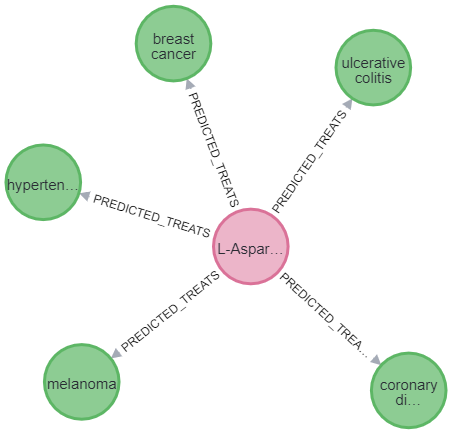
\includegraphics[width=0.45\textwidth]{images/pykeen/predicted treats}
    \caption{5 predicted \textit{treats} relationships for L-Asparagine.}
    \label{fig:predicted_treats}
\end{figure}

\begin{figure}[ht]
    \centering
    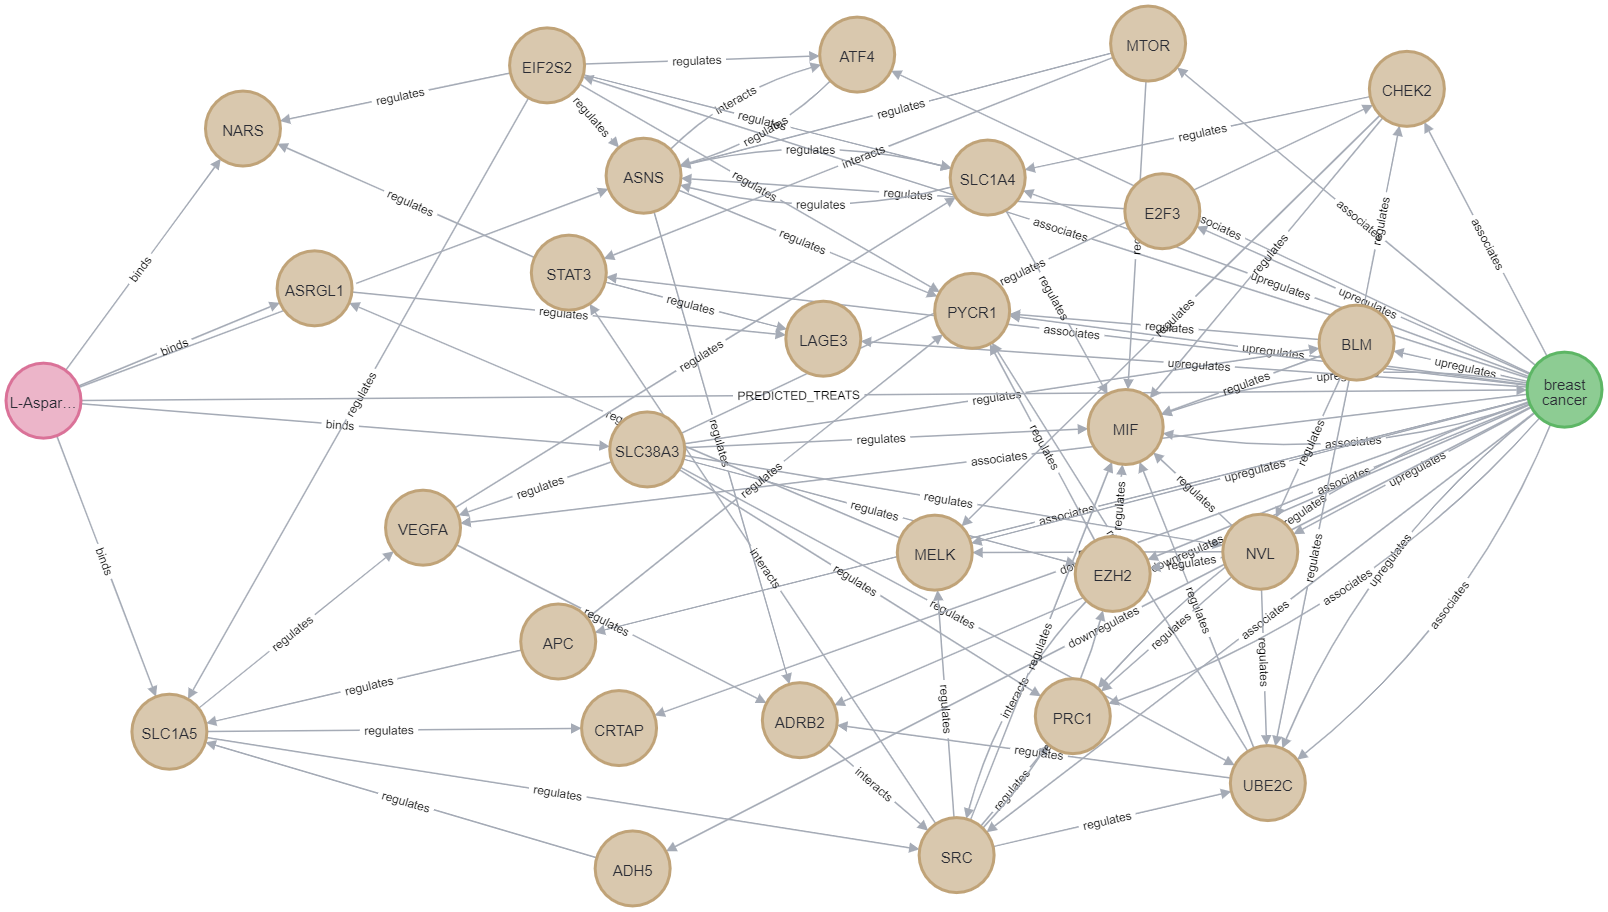
\includegraphics[width=0.8\textwidth]{images/pykeen/results}
    \caption{Visualization of connections between L-Asparagine, genes, and breast cancer, highlighting predicted relationships.}
    \label{fig:kg_visualization}
\end{figure}

\subsection*{Analysis}

The results indicate poor performance across all models tested for knowledge graph completion on the Hetionet dataset.


Among them, RotatE achieved the best results, with the highest MRR ($0.0643$) and Hits@10 ($0.1254$), along with a competitive MR ($1304.77$). The performance of RotatE can be attributed to its use of complex vector space rotations, which enable it to model symmetry, antisymmetry, inversion, and composition—properties that are crucial for representing the diverse and interconnected relationships found in biomedical datasets like Hetionet.

In contrast, the translational models (TransE, TransH, TransR, and TransD) generally underperformed. These models rely on linear transformations (translations) to encode relationships between entities in vector space. While this approach works well for simple, hierarchical relationships, it struggles to handle the multi-relational complexity and semantic diversity present in biomedical knowledge graphs. For instance, TransE achieved an MRR of only 0.0181, and other translational models performed similarly poorly. Their inability to effectively model complex patterns suggests that they are not well-suited for tasks involving heterogeneous biomedical data.

Moreover, the semantic matching models (DistMult, RESCAL, and TuckER) also yielded unsatisfactory results. These models emphasize similarity-based scoring through matrix factorization or tensor decomposition, which may fail to capture the structural dependencies present in Hetionet. Notably, RESCAL performed extremely poorly (MRR = 0.0002), likely due to overfitting caused by its high parameter complexity and a lack of regularization. TuckER, which is tensor-based, fared slightly better but still struggled to effectively utilize the dataset’s structural information, possibly due to insufficient embedding dimensions (128).

Our models, RLM and RLM-A, performed below RotatE, with Hits@10 around $0.11$, indicating they capture relational patterns but lack the rotational expressiveness of RotatE.
Although their mean rank is lower than RotatE, suggesting potential improvements in embedding quality, the addition of retrieval-augmented generation (RAG) did not yield further benefits.

Training losses are shown in Figure~\ref{fig:models_training_losses}, with a performance comparison in Figure~\ref{tab:models_performance_comparison}.

% \subsection{Comparison LLM integration}
% \todo{Fix this mess}

% RLM-A: Llama3.2-3B provided with Wikidata entries to entities
% RLM: Llama3.2-3B embeddings
% RDE: Pipeline with random embeddings
% RotatE:

% Training losses can be seen in \ref{fig:models_training_losses} and \ref{tab:models_performance_comparison}

% RLM-A:
% Hits@1: 0.026036103396710104
% Hits@3: 0.05643381043936481
% Hits@5: 0.07676422416862494
% Hits@10: 0.114104892117069
% Mean Rank: 1216.2593994140625
% Mean Reciprocal Rank: 0.057651162147521966
%
% RLM:
% Hits@1: 0.025849177526169623
% Hits@3: 0.055712810652994375
% Hits@5: 0.07626575518051698
% Hits@10: 0.1131435590685751
% Mean Rank: 1199.255126953125
% Mean Reciprocal Rank: 0.05725240334868432
%
% RDE:
% Hits@1: 0.026036103396710104
% Hits@3: 0.05643381043936481
% Hits@5: 0.07676422416862494
% Hits@10: 0.114104892117069
% Mean Rank: 1216.2593994140625
% Mean Reciprocal Rank: 0.057651162147521966
%
% RotaE
% Hits@1: 0.030424410738446202
% Hits@3: 0.06496119062878303
% Hits@5: 0.08611941892757957
% Hits@10: 0.12543616036459446
% Mean Rank: 1304.7662353515625
% Mean Reciprocal Rank: 0.06425923109054565

% {'TransE': {'hits@1': 0.0027415794345937478, 'hits@3': 0.013084810937833796, 'hits@5': 0.021692302214626504, 'hits@10': 0.039850815352844834, 'mean_rank': 1631.400146484375, 'mean_reciprocal_rank': 0.018126796931028366},
% 'TransH': {'hits@1': 0.003578295236060671, 'hits@3': 0.009506515701773126, 'hits@5': 0.01468703268532365, 'hits@10': 0.02540411592964466, 'mean_rank': 2061.962646484375, 'mean_reciprocal_rank': 0.013518346473574638},
% 'TransR': {'hits@1': 0.00152211066011536, 'hits@3': 0.004788862778608559, 'hits@5': 0.007904293954283274, 'hits@10': 0.015363526312041586, 'mean_rank': 2314.352294921875, 'mean_reciprocal_rank': 0.008869686163961887},
% 'TransD': {'hits@1': 0.006622516556291391, 'hits@3': 0.018737093213700776, 'hits@5': 0.028110090436516414, 'hits@10': 0.046936195969522185, 'mean_rank': 1504.4407958984375, 'mean_reciprocal_rank': 0.02317844331264496}}
% RESCAL
% Hits@1: 0.0
% Hits@3: 8.901231930499181e-06
% Hits@5: 2.6703695791497543e-05
% Hits@10: 0.00012461724702698854
% Mean Rank: 9866.041015625
% Mean Reciprocal Rank: 0.00021927907073404637

% ### TuckER

% Hits@1: 0.004290393790500605
% Hits@3: 0.01131346578366446
% Hits@5: 0.01763334045431888
% Hits@10: 0.03096738588620665
% Mean Rank: 2487.345703125
% Mean Reciprocal Rank: 0.01583893597126007

% DistMult
% "hits_at_1": 0.00641778822188991,
% "hits_at_3": 0.017401908424125898,
% "hits_at_5": 0.025795770134586626,
% "hits_at_10": 0.04272591326639607,
% "mean_rank": 2570.988037109375,
% "mean_reciprocal_rank": 0.02089608460664749,

\begin{table}
    \centering
    \caption{Performance Comparison of Models}
    \label{tab:models_performance_comparison}
    \begin{tabular}{@{}lcccccc@{}}
        \toprule
        \textbf{Model} & \textbf{Hits@1} & \textbf{Hits@3} & \textbf{Hits@5} & \textbf{Hits@10} & \textbf{MR} & \textbf{MRR} \\
        \midrule
        RLM-A          & 0.0260          & 0.0564          & 0.0768          & 0.1141           & 1216.26            & 0.0577                        \\
        RLM            & 0.0258          & 0.0557          & 0.0763          & 0.1131           & \textbf{1199.26}   & 0.0573                        \\
        % RDE            & 0.0260          & 0.0564          & 0.0768          & 0.1141           & 1216.26            & 0.0577                        \\
        RotatE         & \textbf{0.0304} & \textbf{0.0650} & \textbf{0.0861} & \textbf{0.1254}  & 1304.77            & \textbf{0.0643}               \\
        TransE         & 0.0027          & 0.0131          & 0.0217          & 0.0399           & 1631.40            & 0.0181                        \\
        TransH         & 0.0036          & 0.0095          & 0.0147          & 0.0254           & 2061.96            & 0.0135                        \\
        TransR         & 0.0015          & 0.0048          & 0.0079          & 0.0154           & 2314.35            & 0.0089                        \\
        TransD         & 0.0066          & 0.0187          & 0.0281          & 0.0469           & 1504.44            & 0.0232                        \\
        RESCAL         & 0.0000          & 8.9e-6          & 2.7e-5          & 0.0001           & 9866.04            & 0.0002                        \\
        TuckER         & 0.0043          & 0.0113          & 0.0176          & 0.0310           & 2487.35            & 0.0158                        \\
        DistMult       & 0.0064          & 0.0174          & 0.0258          & 0.0427           & 2570.99            & 0.0209                        \\
        \bottomrule
    \end{tabular}
\end{table}


\begin{figure}
    \centering
    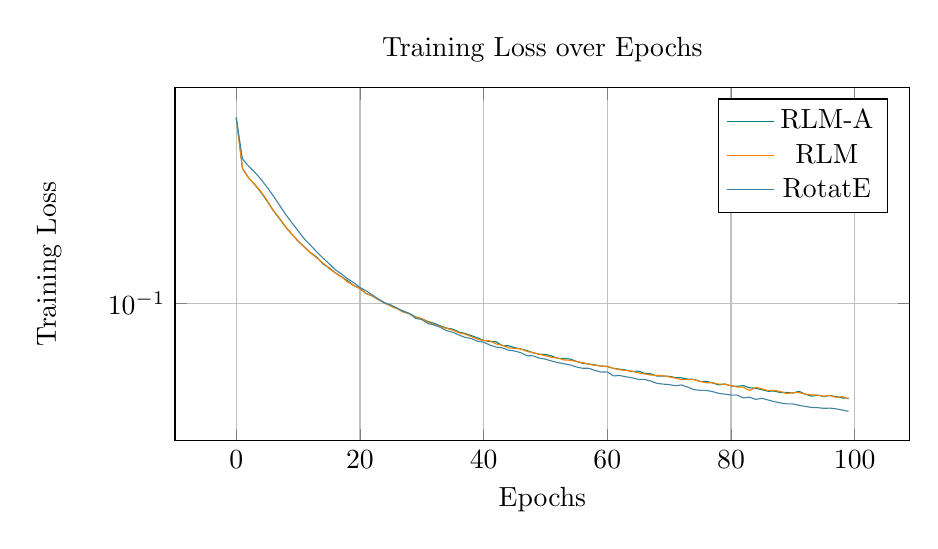
\begin{tikzpicture}
        \begin{axis}[
                xlabel={Epochs},
                ylabel={Training Loss},
                ylabel style={yshift=1em},
                title={Training Loss over Epochs},
                cycle list name=exotic,
                grid=major,
                width=0.9\linewidth,
                height=0.5\linewidth,
                ymode=log,
                legend pos=north east
            ]

            \addplot+[mark=none] coordinates {
                    (00, 0.6215006975894094)
                    (01, 0.3767737554797822)
                    (02, 0.3426325156911359)
                    (03, 0.32072990766147275)
                    (04, 0.297511883232751)
                    (05, 0.27266025224144746)
                    (06, 0.24855261324885766)
                    (07, 0.22963104744978538)
                    (08, 0.2112038403681579)
                    (09, 0.1973995592504536)
                    (10, 0.1839396154894101)
                    (11, 0.17420240018117944)
                    (12, 0.16466365645985398)
                    (13, 0.15757384395612942)
                    (14, 0.14741249475840285)
                    (15, 0.141944090519652)
                    (16, 0.13503937901831434)
                    (17, 0.12994904276450295)
                    (18, 0.12487209878505498)
                    (19, 0.1191292264772439)
                    (20, 0.11567145115897433)
                    (21, 0.11018701893932999)
                    (22, 0.10751756815269488)
                    (23, 0.10388408314462132)
                    (24, 0.10029823847267785)
                    (25, 0.0974403634871057)
                    (26, 0.09493673855867364)
                    (27, 0.09282103720585687)
                    (28, 0.09040026507575855)
                    (29, 0.08761885351499284)
                    (30, 0.08594255543956723)
                    (31, 0.08373290048339373)
                    (32, 0.08219589875132728)
                    (33, 0.08018838834009029)
                    (34, 0.07848552661971242)
                    (35, 0.07763778672029598)
                    (36, 0.07551116908737086)
                    (37, 0.07446351479357087)
                    (38, 0.07284486955689407)
                    (39, 0.0713551490395786)
                    (40, 0.06948803136112479)
                    (41, 0.06878861424286165)
                    (42, 0.06857837627987655)
                    (43, 0.06604571190741176)
                    (44, 0.0659427966897064)
                    (45, 0.06479331085581443)
                    (46, 0.06390419534507265)
                    (47, 0.06294223639884951)
                    (48, 0.06155227326654356)
                    (49, 0.06073843196441753)
                    (50, 0.06057692843580572)
                    (51, 0.05968840565354243)
                    (52, 0.058315730320633405)
                    (53, 0.05820704163274895)
                    (54, 0.05789005863299945)
                    (55, 0.05658578239635889)
                    (56, 0.05551888389780201)
                    (57, 0.055188916954540715)
                    (58, 0.05464516315346155)
                    (59, 0.05403509550220874)
                    (60, 0.053750831574405245)
                    (61, 0.05282256083567213)
                    (62, 0.05239069027346739)
                    (63, 0.05198787114580834)
                    (64, 0.05121267382437385)
                    (65, 0.051436112205029076)
                    (66, 0.05032967896559244)
                    (67, 0.05008214164805304)
                    (68, 0.049019652331812234)
                    (69, 0.04903715261701571)
                    (70, 0.048860486698653)
                    (71, 0.048284420968459786)
                    (72, 0.04813197712522161)
                    (73, 0.04756473994268643)
                    (74, 0.047434608840249935)
                    (75, 0.04647610245319189)
                    (76, 0.04650410510820245)
                    (77, 0.04577165995650248)
                    (78, 0.044940628645971314)
                    (79, 0.045329166830841934)
                    (80, 0.044480651714637505)
                    (81, 0.04430044092373723)
                    (82, 0.044607484925343124)
                    (83, 0.04367613100397967)
                    (84, 0.04345479718746791)
                    (85, 0.04286472234611902)
                    (86, 0.04220358264507357)
                    (87, 0.04227263889443087)
                    (88, 0.041648908600991845)
                    (89, 0.041692908110780164)
                    (90, 0.04146903044287463)
                    (91, 0.04215777642889148)
                    (92, 0.04102023117295159)
                    (93, 0.04021583949396035)
                    (94, 0.04060482946574552)
                    (95, 0.04008542710240583)
                    (96, 0.04050048666842842)
                    (97, 0.0400221950092389)
                    (98, 0.03951605528185742)
                    (99, 0.03941562074259908)
                };
            \addlegendentry{RLM-A}

            \addplot+[mark=none] coordinates {
                    (00, 00.6186414349459298)
                    (01, 00.37638175582559885)
                    (02, 00.34275079744280335)
                    (03, 00.32128739553866464)
                    (04, 00.29979521287329375)
                    (05, 00.2743557864006668)
                    (06, 00.24939728319509155)
                    (07, 00.23069555001812805)
                    (08, 00.21186267508189607)
                    (09, 00.197036191956872)
                    (10, 0.18473960819032578)
                    (11, 0.17368744683700163)
                    (12, 0.1641184890256656)
                    (13, 0.156514597882714)
                    (14, 0.1487770409478142)
                    (15, 0.14088273946204327)
                    (16, 0.13490956745074387)
                    (17, 0.1298277757399989)
                    (18, 0.12347863343011817)
                    (19, 0.11933057376762729)
                    (20, 0.11558022611437191)
                    (21, 0.11015828539339448)
                    (22, 0.10763842997762771)
                    (23, 0.10354924152747373)
                    (24, 0.10066375935742958)
                    (25, 0.09741394131832623)
                    (26, 0.0948367329793802)
                    (27, 0.09176234300152859)
                    (28, 0.09020200588980133)
                    (29, 0.0872251197763619)
                    (30, 0.08609596755279224)
                    (31, 0.08332153993546283)
                    (32, 0.08118542629147717)
                    (33, 0.0797906739039003)
                    (34, 0.07819930132232386)
                    (35, 0.0769997337888205)
                    (36, 0.07494410485504428)
                    (37, 0.07394385077313845)
                    (38, 0.07215340544123856)
                    (39, 0.0704387085075259)
                    (40, 0.06937430027643206)
                    (41, 0.06924111737205661)
                    (42, 0.06714219749313281)
                    (43, 0.06639708262064191)
                    (44, 0.0646502775031912)
                    (45, 0.06426771735276068)
                    (46, 0.06390810454081837)
                    (47, 0.0624039978264133)
                    (48, 0.06163813514053686)
                    (49, 0.06064767948010245)
                    (50, 0.05981564248545023)
                    (51, 0.05886537351715537)
                    (52, 0.0585007877481554)
                    (53, 0.057371103062648705)
                    (54, 0.057211875296059936)
                    (55, 0.05651157429115104)
                    (56, 0.05593476105048607)
                    (57, 0.054984153258977014)
                    (58, 0.05442626859169614)
                    (59, 0.054027240341508034)
                    (60, 0.05389867955924846)
                    (61, 0.05282311574269536)
                    (62, 0.052101299557028705)
                    (63, 0.05175519572541219)
                    (64, 0.05139087534303817)
                    (65, 0.050517770765107425)
                    (66, 0.05003554361250786)
                    (67, 0.049473038651812865)
                    (68, 0.04935508802668923)
                    (69, 0.04915398142060821)
                    (70, 0.048589498483510116)
                    (71, 0.048017211682704154)
                    (72, 0.04725801281138813)
                    (73, 0.0473098272334674)
                    (74, 0.047289202647423687)
                    (75, 0.0464604841439151)
                    (76, 0.04586672304720026)
                    (77, 0.04591426782411839)
                    (78, 0.04528597391004714)
                    (79, 0.04518300194743011)
                    (80, 0.044598239081527755)
                    (81, 0.04399099294308378)
                    (82, 0.04389825539243384)
                    (83, 0.04246989421223997)
                    (84, 0.04384734970358347)
                    (85, 0.04320053129556646)
                    (86, 0.04245398653955421)
                    (87, 0.04254348554854241)
                    (88, 0.042123571687414055)
                    (89, 0.041276223329585346)
                    (90, 0.04159939016697076)
                    (91, 0.04161881064414842)
                    (92, 0.04104187161341343)
                    (93, 0.04073595737609885)
                    (94, 0.040613451942903306)
                    (95, 0.040189360503896494)
                    (96, 0.0404375596205303)
                    (97, 0.03976845748909242)
                    (98, 0.04001958809945741)
                    (99, 0.0391153971959491)
                };
            \addlegendentry{RLM}

            %\addplot+[mark=none] coordinates {
            %(00, 0.6215006975894094)
            %(01, 0.3767737554797822)
            %(02, 0.3426325156911359)
            %(03, 0.32072990766147275)
            %(04, 0.297511883232751)
            %(05, 0.27266025224144746)
            %(06, 0.24855261324885766)
            %(07, 0.22963104744978538)
            %(08, 0.2112038403681579)
            %(09, 0.1973995592504536)
            %(10, 0.1839396154894101)
            %(11, 0.17420240018117944)
            %(12, 0.16466365645985398)
            %(13, 0.15757384395612942)
            %(14, 0.14741249475840285)
            %(15, 0.141944090519652)
            %(16, 0.13503937901831434)
            %(17, 0.12994904276450295)
            %(18, 0.12487209878505498)
            %(19, 0.1191292264772439)
            %(20, 0.11567145115897433)
            %(21, 0.11018701893932999)
            %(22, 0.10751756815269488)
            %(23, 0.10388408314462132)
            %(24, 0.10029823847267785)
            %(25, 0.0974403634871057)
            %(26, 0.09493673855867364)
            %(27, 0.09282103720585687)
            %(28, 0.09040026507575855)
            %(29, 0.08761885351499284)
            %(30, 0.08594255543956723)
            %(31, 0.08373290048339373)
            %(32, 0.08219589875132728)
            %(33, 0.08018838834009029)
            %(34, 0.07848552661971242)
            %(35, 0.07763778672029598)
            %(36, 0.07551116908737086)
            %(37, 0.07446351479357087)
            %(38, 0.07284486955689407)
            %(39, 0.0713551490395786)
            %(40, 0.06948803136112479)
            %(41, 0.06878861424286165)
            %(42, 0.06857837627987655)
            %(43, 0.06604571190741176)
            %(44, 0.0659427966897064)
            %(45, 0.06479331085581443)
            %(46, 0.06390419534507265)
            %(47, 0.06294223639884951)
            %(48, 0.06155227326654356)
            %(49, 0.06073843196441753)
            %(50, 0.06057692843580572)
            %(51, 0.05968840565354243)
            %(52, 0.058315730320633405)
            %(53, 0.05820704163274895)
            %(54, 0.05789005863299945)
            %(55, 0.05658578239635889)
            %(56, 0.05551888389780201)
            %(57, 0.055188916954540715)
            %(58, 0.05464516315346155)
            %(59, 0.05403509550220874)
            %(60, 0.053750831574405245)
            %(61, 0.05282256083567213)
            %(62, 0.05239069027346739)
            %(63, 0.05198787114580834)
            %(64, 0.05121267382437385)
            %(65, 0.051436112205029076)
            %(66, 0.05032967896559244)
            %(67, 0.05008214164805304)
            %(68, 0.049019652331812234)
            %(69, 0.04903715261701571)
            %(70, 0.048860486698653)
            %(71, 0.048284420968459786)
            %(72, 0.04813197712522161)
            %(73, 0.04756473994268643)
            %(74, 0.047434608840249935)
            %(75, 0.04647610245319189)
            %(76, 0.04650410510820245)
            %(77, 0.04577165995650248)
            %(78, 0.044940628645971314)
            %(79, 0.045329166830841934)
            %(80, 0.044480651714637505)
            %(81, 0.04430044092373723)
            %(82, 0.044607484925343124)
            %(83, 0.04367613100397967)
            %(84, 0.04345479718746791)
            %(85, 0.04286472234611902)
            %(86, 0.04220358264507357)
            %(87, 0.04227263889443087)
            %(88, 0.041648908600991845)
            %(89, 0.041692908110780164)
            %(90, 0.04146903044287463)
            %(91, 0.04215777642889148)
            %(92, 0.04102023117295159)
            %(93, 0.04021583949396035)
            %(94, 0.04060482946574552)
            %(95, 0.04008542710240583)
            %(96, 0.04050048666842842)
            %(97, 0.0400221950092389)
            %(98, 0.03951605528185742)
            %(99, 0.03941562074259908)
            %};
            %\addlegendentry{RDE}

            \addplot+[mark=none] coordinates {
                    (00, 0.6171451922429722)
                    (01, 0.41325790233112414)
                    (02, 0.3845483400012475)
                    (03, 0.3623269587958864)
                    (04, 0.33810757640282496)
                    (05, 0.31246766190050945)
                    (06, 0.2869352645374376)
                    (07, 0.26201090349015993)
                    (08, 0.23949873430446503)
                    (09, 0.2204936422017278)
                    (10, 0.20383941696146354)
                    (11, 0.18846062864420898)
                    (12, 0.17700284926522022)
                    (13, 0.1659027688324044)
                    (14, 0.15620337253551006)
                    (15, 0.14781650130325136)
                    (16, 0.13922729976220663)
                    (17, 0.13352018077104671)
                    (18, 0.12729803000943807)
                    (19, 0.1225688527412458)
                    (20, 0.11685701199979065)
                    (21, 0.11311606792966435)
                    (22, 0.10864997166368033)
                    (23, 0.1042215110975952)
                    (24, 0.10063370456388708)
                    (25, 0.09853136603951726)
                    (26, 0.0954483598810122)
                    (27, 0.09241732165794438)
                    (28, 0.09051212892445454)
                    (29, 0.08633690665142954)
                    (30, 0.08529175563390815)
                    (31, 0.082023410003522)
                    (32, 0.08082775360902512)
                    (33, 0.07909642996644105)
                    (34, 0.0764937254267157)
                    (35, 0.075379783427661)
                    (36, 0.07334772887764868)
                    (37, 0.07162315983978654)
                    (38, 0.07080203338880474)
                    (39, 0.06900147586246286)
                    (40, 0.06831186605036123)
                    (41, 0.06641652615813025)
                    (42, 0.06514142545317735)
                    (43, 0.06461050195072127)
                    (44, 0.06320943232786955)
                    (45, 0.06263272075623207)
                    (46, 0.06166005668342792)
                    (47, 0.05983979131067532)
                    (48, 0.059752607883584254)
                    (49, 0.05843401587396385)
                    (50, 0.057825785910961026)
                    (51, 0.05677372303734065)
                    (52, 0.0559254687678298)
                    (53, 0.05524666137263552)
                    (54, 0.054632422329692475)
                    (55, 0.05354685106384727)
                    (56, 0.05286392320906383)
                    (57, 0.052870493942281924)
                    (58, 0.0517646087448119)
                    (59, 0.05092644081334318)
                    (60, 0.0510308629152172)
                    (61, 0.049057520832654286)
                    (62, 0.04925112097878391)
                    (63, 0.04863642670366922)
                    (64, 0.048191811197812844)
                    (65, 0.04741993217659024)
                    (66, 0.04742957783145894)
                    (67, 0.04665702909808224)
                    (68, 0.04562084779890089)
                    (69, 0.04526589787512135)
                    (70, 0.04505183628350836)
                    (71, 0.04455140070535735)
                    (72, 0.04487727565482972)
                    (73, 0.043940447092667256)
                    (74, 0.042856323042702024)
                    (75, 0.04258967153218857)
                    (76, 0.04253054668613474)
                    (77, 0.042069480272862794)
                    (78, 0.04133290488586882)
                    (79, 0.04104606414336821)
                    (80, 0.04064872705617364)
                    (81, 0.040640457717867264)
                    (82, 0.03952631749772808)
                    (83, 0.03984648186144905)
                    (84, 0.038959588435455175)
                    (85, 0.039407932702324656)
                    (86, 0.038721918185710365)
                    (87, 0.03812627882563036)
                    (88, 0.037613779187609775)
                    (89, 0.03730773910931004)
                    (90, 0.037262268114096754)
                    (91, 0.03679166536498178)
                    (92, 0.03635163325179954)
                    (93, 0.03602182241008195)
                    (94, 0.03593000490006255)
                    (95, 0.03569717517712393)
                    (96, 0.03575632047833099)
                    (97, 0.035496792015630184)
                    (98, 0.03511317789232134)
                    (99, 0.03465121926777998)
                };
            \addlegendentry{RotatE}


        \end{axis}
    \end{tikzpicture}
    \caption{Logarithmic plot of training loss.}
    \label{fig:models_training_losses}
\end{figure}


\section*{Discussion}

Comparison with expectations, limitations, lessons learned, and perspectives.


\bibliography{main}

\end{document}
